\documentclass[convert={size=250}]{standalone}

\usepackage{tikz}
\usepackage{tikz-qtree}

\begin{document}

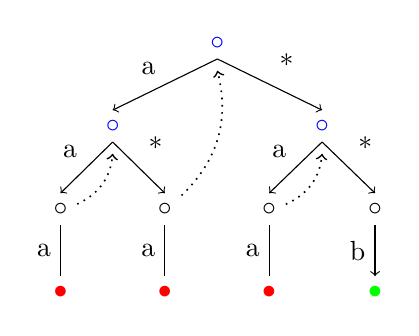
\begin{tikzpicture}[sibling distance=20pt, level distance=30pt]
    \Tree [.\node[blue](/){$\circ$};
        \edge[->] node[auto=right] {a};
        [.\node[blue](/a){$\circ$};
            \edge[->] node[auto=right] {a};
            [.\node(/a/a){$\circ$};
                \edge node[auto=right] {a};
                [.\node[red](/a/a/a){$\bullet$}; ]
                ]
            \edge[->] node[auto=left] {*};
            [.\node(/a/*){$\circ$};
                \edge node[auto=right] {a};
                [.\node[red](/a/*/a){$\bullet$}; ] ] ]
        \edge[->] node[auto=left] {*};
        [.\node[blue](/*){$\circ$};
            \edge[->] node[auto=right] {a};
            [.\node(/*/a){$\circ$};
                \edge node[auto=right] {a};
                [.\node[red](/*/a/a){$\bullet$}; ] ]
            \edge[->] node[auto=left] {*};
            [.$\circ$
                \edge[->] node[auto=right] {b};
                [.\node[green]{$\bullet$}; ] ] ] ]

    \draw[semithick,->,dotted] (/a/a) to[bend right] ([yshift=-10pt]/a);
    \draw[semithick,->,dotted] (/a/*) to[bend right] ([yshift=-10pt]/);
    \draw[semithick,->,dotted] (/*/a) to[bend right] ([yshift=-10pt]/*);
\end{tikzpicture}

\end{document}

